
\chapter{Advanced programming techniques}

\begin{tcolorbox}
  Normal pragramming techniques enable us to build ``standard Python toolbox'' and
  advanced programming techniques can bring us ``deluxe Python toolbox''.
\end{tcolorbox}

\section{Further procedural programming}

\subsection{Branching using dictionaries}


\begin{tcolorbox}
  Functions are objects like everything else in Python, and
  a function's name is an object reference that refers to the function.
  If we write a function's name without parentheses,
  Python knows we mean the object reference, and
  we can pass such object references around like any others.
\end{tcolorbox}

We can use this fact to produce \verb|if| statements that have lots of \verb|elif| clauses with a single function call.


\begin{lstlisting}
# (A)dd (E)dit (L)ist (R)emove (I)mport e(X)port (Q)uit
if action == "a":
    add_dvd(db)
elif action == "e":
    edit_dvd(db)
elif action == "l":
    list_dvds(db)
elif action == "r":
    remove_dvd(db)
elif action == "i":
    import_(db)
elif action == "x":
    export(db)
elif action == "q":
    quit(db)

# The same effect
# (A)dd (E)dit (L)ist (R)emove (I)mport e(X)port (Q)uit
functions = dict(a=add_dvd, e=edit_dvd, l=list_dvds, r=remove_dvd,
              i=import_, x=export, q=quit)
functions[action](db)  
\end{lstlisting}

Not only is the code on the bottom much shorter than the code on the top,
but also it can scale (have far more dictionary items) without affecting its performance,
unlike the upper code whose speed depends on how many \verb|elif|s must be tested to find the appropriate function to call.


\begin{lstlisting}
    def import_(self, filename, reader=None):
        extension = os.path.splitext(filename)[1].lower()
        call = {
            ('.aix', 'dom'): self.import_xml_dom,
            ('.aix', 'etree'): self.import_xml_etree,
            ('.aix', 'sax'): self.import_xml_sax,
            ('.ait', 'manual'): self.import_text_manual,
            ('ait', 'regex'): self.import_text_regex,
            ('.aib', None): self.import_binary,
            ('.aip', None): self.import_pickle
        }
        result = call[extension, reader](filename)
        if not result:
            self.clear()
        return result  
\end{lstlisting}


\subsection{Generator expressions and functions}

Generator expression:
\begin{tcolorbox}
\begin{verbatim}
(expression for item in iterable)
(expression for item in iterable if condition)
\end{verbatim}
\end{tcolorbox}

\begin{lstlisting}
def items_in_key_order(d):
    for key in sorted(d):
        yield key, d[key]  # yield


def items_in_key_order2(d):
    return ((key, d[key]) for key in sorted(d))  # generator expression
  
\end{lstlisting}

Both functions return a generator.
If we need all the items in one go
we can pass the generator returned to \verb|list()| or \verb|tuple()|.



Generator provide a means of performing lazy evaluation,
which means that they compute only the values that are actually needed.
This can be more efficient than, say, computing a very large list in one go.
Some generator produce as many values as we ask for -- without any upper limit.
For example
\begin{lstlisting}
def quarters(next_quarter=0.0):
    while True:
        yield next_quarter
        next_quarter += 0.25
\end{lstlisting}

This function will return 0.0, 0.25, 0.5, and so on, forever.
Here is how we could use the generator:
\begin{lstlisting}
result = []
for x in quarters():
    result.append(x)
    if x >= 1.0:
        break  
# [0.0, 0.25, 0.5, 0.75, 1.0]
\end{lstlisting}


\begin{lstlisting}
def quarters(next_quarter=0.0):
    while True:
        received = (yield next_quarter)
        if received is None:
            next_quarter += 0.25
        else:
            next_quarter = received


result = []
generator = quarters()
while len(result) < 5:
    x = next(generator)
    if abs(x - 0.5) < sys.float_info.epsilon:
        x = generator.send(1.0)  # Notice this
    result.append(x)
print(result)  # [0.0, 0.25, 1.0, 1.25, 1.5]  
\end{lstlisting}

We create a variable to refer to the generator and
call the built-in \verb|next()| function which retrieves the next item from the generator it is given.
(The same effect can be achieved by calling the \verb|generator’s __next__()| special method,
in this case, \verb|x = generator.__next__()|.)
If the value is equal to 0.5 we send the value 1.0 into the generator (which immediately yields this value back). 



\subsection{Dynamic code execution and dynamic imports}

\subsubsection{Dynamic code execution}

There are two built-in functions for dynamic code execution:
\begin{description}
\item[eval()] for expression
\item[exec()] for code
\end{description}


\begin{lstlisting}
import math

x = eval('2 ** 10')
print(x)  # 1024

code = '''
def area_of_sphere(r):
    return 4 * math.pi * r ** 2
'''
# context = {}
# context['math'] = math
# exec(code, context)  # define the function area_of_sphere
context = globals().copy()
exec(code, context)

area_of_sphere = context['area_of_sphere']
sphere = area_of_sphere(5)
print(sphere)  # 314.1592653589793  
\end{lstlisting}


If \verb|exec()| is called with some code as its only argument there is no way to access any functions or variables
that are created as a result of the code bing executed.
Furthermore, \verb|exec()| cannot access any imported modules or any of the variables, functions, or the objects
that are in scope at the point of the call.
Both of these problems can be solved by passing a dictionary as the second argument.
The dictionary provides a place where object references can be kept for accessing after the \verb|exec()| call has finished.
For example, the use of the \verb|context| dictionary means that
after the \verb|exec()| call,
the dictionary has an object reference to the \verb|area_of_sphere()| function that was created by \verb|exec()|.
In this example we needed \verb|exec()| to be able to access the \verb|math| module,
so we inserted an item into the context dictionary whose key is the module’s name and
whose value is an object reference to the corresponding module object.
This ensures that inside the \verb|exec()| call, \verb|math.pi| is accessible.



\subsubsection{Dynamic importing modules}

Python provides three straightforward mechanisms that can be used to create plug-ins,
all of which involve importing modules by name at runtime.
And once we have dynamically imported additional modules,
we can use Python’s introspection functions to check the availability of the functionality we want,
and to access it as required.


The main function is:
\begin{lstlisting}
def main():
    modules = load_modules()
    get_file_type_functions = []
    for module in modules:
        get_file_type = get_function(module, 'get_file_type')
        if get_file_type is None:
            get_file_type_functions.append(get_file_type)

    for file in get_files(sys.argv[1:]):
        fh = None
        try:
            fh = open(file, 'rb')
            magic = fh.read(1000)
            for get_file_type in get_file_type_functions:
                filetype = get_file_type(magic, os.path.splitext(file)[1])  # file extension
                if filetype is not None:
                    print(f'{filetype:.<20}{file}')
                    break
            else:
                print('{:.<20}{}'.format('Unknown', file))
        except EnvironmentError as err:
            print(err)
        finally:
            if fh is not None:
                fh.close()  
\end{lstlisting}


The longest and most difficult approach (approach 1):
\begin{lstlisting}
def load_modules():
    modules = []
    for name in os.listdir(os.path.dirname(__file__) or '.'):
        if name.endswith('.py') and 'magic' in name.lower():
            filename = name
            name = os.path.splitext(name)[0]  # remove extension
            if name.isidentifier() and name not in sys.modules:
                fh = None
                try:
                    fh = open(filename)
                    code = fh.read()
                    module = type(sys)(name)
                    sys.modules[name] = module
                    exec(code, module.__dict__)
                    modules.append(module)
                except (EnvironmentError, SyntaxError) as err:
                    sys.modules.pop(name, None)
                    print(err)
                finally:
                    if fh is not None:
                        fh.close()
    return modules  
\end{lstlisting}
      
We begin by iterating over all the files in the program's directory.
If this the current directory, \verb|os.path.dirname(__file__)| will return an empty string
which would cause \verb|os.listdir()| to raise an exception,
so we pass \verb|"."| if necessary.


The line \verb|module = type(sys)(name)| is quite subtle.
When we call \verb|type()| it returns the type object of the object it is given.
So if we called \verb|type(1)| we would get \verb|int| back.
If we call the type object as a function, we get an object of that type back.
For example, we can get the interger 5 in variable \verb|x| by writting \verb|x = 5|, or \verb|x = int(5)|,
or \verb|x = type(0)(5)|.
In this case we've used \verb|type(sys)| and \verb|sys| is a module,
so we get back the module type object, can
can be used to create a new module with the given name.
Just as with the \verb|int| example where it didn't matter what integer we used to get the \verb|int| type object,
it doesn't matter what module we use to get the module type object.


Once we have a new module, we add it to the global list of modules to preven the module from accidentally reimported.
This is done before calling \verb|exec()| to more closely mimic the behavior of the \verb|import| statement.


The second way to dynamically load a module at runtime (approch 2) --
the code shown here replaces the first approach’s \verb|try ... except| block:
\begin{lstlisting}
                try:
                    exec('import ' + name)
                    modules.append(sys.modules[name])
                except SyntaxError as err:
                    print(err)  
\end{lstlisting}

One theoretical problem with this approach is that it is potentially insecure.
The name variable could begin with \verb|sys|; and be followed by some destructive code.


The easiest way to dynamically import module and is slightly safer than using \verb|exec()| (approach 3):
\begin{lstlisting}
                try:
                    module = __import__(name)
                    modules.append(module)
                except SyntaxError as err:
                    print(err)  
\end{lstlisting}





Having imported the module we need to be able to access the functionality it provides.
This can be achieved using Python's built-in introspection functions, \verb|getattr()| and \verb|hasattr()|.

\begin{lstlisting}
def get_function(module, function_name):
    function = get_function.cache.get((module, function_name), None)
    if function is None:
        try:
            function = getattr(module, function_name)
            if not hasattr(function, '__call__'):
                raise AttributeError()
            get_function.cache[(module, function_name)] = function
        except AttributeError:
            function = None
    return function  
\end{lstlisting}

Ignoring the cache-related code for a moment,
what the function does is call \verb|getattr()| on the module object with the name of the function we want.
If there is no such attribute an \verb|AttributeError| exception is raised,
but if there is such an attribute we use \verb|hasattr()| to check that
the attribute itself has the \verb|__call__| attribute --
something that all callables (functions and methods) have.
If the attribute exists and is callable we can return it to the caller;
otherwise, we return \verb|None| to signify that the function isn’t available.



If hundreds of files were being processed (e.g. *.*),
we don't want to go throught the lookup process for every module for every file.
So immediately after defining the \verb|get_function()| function,
we add an attribute to the function, a dictionary called \verb|cache|.
(In general, Python allows us to add arbitrary attributes to arbitrary objects.)
The first time that \verb|get_function()| is called the cache dictionary is empty,
so the \verb|dict.get(|) call will return None.
But each time a suitable function is found
it is put in the dictionary with a 2-tuple of the module and function name used as the key and
the function itself as the value.
So the second and all subsequent times a particular function is requested
the function is immediately returned from the cache and no attribute lookup takes place at all.




The technique used for caching the \verb|get_function()|'s return value for a given set of arguments is called \keyword{memorizing}.
It can be used for any function that has no \keyword{side effects} (does not change any global variables), and
that always returns the same result for the same (immutable) arguments.

\newpage

\begin{tcolorbox}
\keyword{Dynamic programming and introspection functions:}
\begin{description}
\item[\_{}\_{}import\_{}\_{}(...)] Imports a module by name
\item[compile(source, file, mode)] Returns the code object that results from compiling the \verb|source| text;
  \verb|file| must be the filename, or ``<string>'';
  \verb|mode| must be ``single'', ``eval'', or ``exec''
\item[delattr(obj, name)] Deletes the attribute called \verb|name| from object \verb|obj|
\item[getattr(obj, name, val)] Returns the value of the attribute called \verb|name| from object \verb|obj|,
  or \verb|val| if given and there is no such attribute
\item[hasattr(obj, name)] Returns \verb|True| if object \verb|obj| has an attribute called \verb|name|
\item[setattr(obj, name, val)] Sets the attribute called \verb|name| to the value \verb|val| for the object \verb|obj|,
  creating the attribute if necessary
\item[eval(source, globals, locals)] Returns the result of evaluating the single expression in \verb|source|;
  if supplied, \verb|globals| is the global context and
  \verb|locals| is the local context (as dictionaries)
\item[exec(obj, globals, locals)] Evaluates object \verb|obj|, which can be a string or a code object from \verb|compile()|,
  and returns None;
  if supplied, \verb|globals| is the global context and \verb|locals| is the local context
\item[dir(obj)] Returns the list of names in the local scope, or if \verb|obj| is given then \verb|obj|'s names
\item[globals()] Returns a dictionary of the current global context
\item[locals()] Returns a dictionary of the current local context
\item[type(obj)] Returns object \verb|obj|'s type object
\item[vars(obj)] Returns object \verb|obj|'s context as a dictionary;
  or the local context if obj is not given
\end{description}
\end{tcolorbox}


\subsection{Local and recursive functions}

Functions defined inside the definition of an existing function are called \keyword{nested functions} or \keyword{local functions.}


One common use case for local functions is when we want to use recursion.
Recursive functions can be \keyword{computationally expensive}
because for every recursive call another stack frame is used;
however, some algorithms are most naturally expressed using recursion.
Most Python implementations have a fixed limit to how many recursive calls can be made.
The limit is returned by \verb|sys.getrecursionlimit()| and can be changed by \verb|sys.setrecursionlimit()|,
although increasing the limit is most often a sign that the algorithm being used is inappropriate or that
the implementation has a bug.


\subsection{Functions and method decorators}

\begin{tcolorbox}
  A decorator is a function that takes a function or method as its sole argument and
  returns a new function or method that incorporates the docorated function or method
  with some additional functionality added.
\end{tcolorbox}


\begin{lstlisting}
@positive_result
def discriminant(a, b, c):
    return b ** 2 - 4 * a * c
\end{lstlisting}


Here's the decorator's implementation:
\begin{lstlisting}
def positive_result(function):
    def wrapper(*args, **kwargs):
        result = function(*args, **kwargs)
        assert result >= 0, function.__name__ + "() result isn't >= 0"
        return result

    wrapper.__name__ = function.__name__
    wrapper.__doc__ = function.__doc__
    return wrapper
\end{lstlisting}


Docorator define a new local function (here \verb|wrapper()|) tha calls the original function.
The wrapper finishes by returning the result computed by the wrapped function.
After creating the wrapper, we set its name and docstring to those of the original function.
\keyword{This helps with introspection,
  since we want error messages to mention the name of the original function, not the wrapper.}
Finally, we return the wrapper function -- it is this function that will be used in place of the original.




Here is slightly cleaner version:
\begin{lstlisting}
import functools
  
def positive_result(function):
    @functools.wraps(function)
    def wrapper(*args, **kwargs):
        result = function(*args, **kwargs)
        assert result >= 0, function.__name__ + "() result isn't >=0"
        return result

    return wrapper  
\end{lstlisting}

The wrapper itself is wrapped using the \verb|functools| module's \verb|@functools.wraps| decorator,
which ensures that the \verb|wrapper()| function has the name and docstring of the original function.


In some cases it would be useful to be able to parameterize a decorator.
(At first sight this does not seem possible since a decorator takes just one argument, a function or method.
But there is a neat solution to this.
We can call a function with the parameters we want and that returns a decorator
which can then decorate the function that follows it.)
For example:
\begin{lstlisting}
@bounded(0, 100)
def percent(amount, total):
    return (amount / total) * 100  
\end{lstlisting}

Here's the implementation of the \verb|bounded()| function:
\begin{lstlisting}
def bounded(minimum, maximum):
    def decorator(function):
        @functools.wraps(function)
        def wrapper(*args, **kwargs):
            result = function(*args, **kwargs)
            if result < minimum:
                return minimum
            elif result > maximum:
                return maximum
            return result

        return wrapper

    return decorator  
\end{lstlisting}


Here is a log decorator:
\begin{lstlisting}
import logging
import functools
import os
import tempfile


def logged(file):
    """
    Log the output of the decorated function into a logged file.

    :param file: If file is None, use temple file, otherwise use the given file
    :return: decorated function
    """
    def decorator(function):
        if __debug__:
            logger = logging.getLogger('Logger')
            logger.setLevel(logging.DEBUG)
            if file is None:
                handler = logging.FileHandler(os.path.join(tempfile.gettempdir(), 'logged.log'))
            else:
                handler = logging.FileHandler(file)
            logger.addHandler(handler)

            @functools.wraps(function)
            def wrapper(*args, **kwargs):
                # accumulate string
                log = 'called: ' + function.__name__ + '('
                log += ', '.join([f'{a!r}' for a in args] + [f'{k!s}={v!r}' for k, v in kwargs.items()])
                result = exception = None
                try:
                    result = function(*args, **kwargs)
                    return result
                except Exception as err:
                    exception = err
                finally:
                    log += (') -> ' + str(result)) if exception is None else f'{type(exception)}: {exception}'
                    logger.debug(log)
                    if exception is not None:
                        raise exception

            return wrapper
        else:
            return function

    return decorator


@logged(None)
def say_word(word='hello'):
    return word  
\end{lstlisting}

\subsection{Function annotations}

Functions and methods can be defined with annotations --- expressions that can be used in a function's signature.

\begin{tcolorbox}
  General syntax:
\begin{verbatim}
def functionName(par: exp1, par2: exp2, ..., parN: expN) -> rexp:
    suite
\end{verbatim}
\end{tcolorbox}

Every colon expression part (\verb|: expX|) is an optional annoation,
and so is the arrow return expression part (\verb|-> rexp|).


If annoations are present they are added to the function's \verb|__annotations__| dictionary;
if they are not present this dictionary is empty.
The dictionary's keys are the parameter names, and the value are the corresponding expressions.
The syntax allows us to annoate all, some, or none of the parameters and to annoate the return value or not.
Annotations have no special significance to Python.
\keyword{The only thing that Python does in the face of annotations is to put them in the \_{}\_{}annotations\_{}\_{} dictionary}; any other action is up to us.



\begin{lstlisting}
def is_unicode_punctuations(s: str) -> bool:
    for c in s:
        # print(unicodedata.category(c))

        # Every Unicode character belongs to a particular category and each category is
        # identified by a two-character identifier. All the categories that begin with P are
        # punctuation characters.
        if unicodedata.category(c)[0] != 'P':
            return False
    return True


print(is_unicode_punctuations.__annotations__)
# {'s': <class 'str'>, 'return': <class 'bool'>}
\end{lstlisting}


If we want to give meaning to annotations, for example, to provide type checking,
one approach is to decorate the functions we want the meaning to apply to with a suitable decorator.
Here is a very basic type-checking decorator:

\begin{lstlisting}
import inspect
import functools

def strictly_typed(function):
    """
    # This decorator requires that every argument and the return value must be
    # annotated with the expected type.
    # Notice that the checking is done only in debug mode (which is Python’s default
    # mode —- controlled by the -O command-line option and the PYTHONOPTIMIZE environment variable).

    :param function:
    :return: decorated function
    """
    annotations = function.__annotations__
    arg_spec = inspect.getfullargspec(function)

    # assert all type is given
    assert 'return' in annotations, 'missing type for return value'
    # arg_spec.args: positional arguments
    # kwonlyargs: keyword only arguments (kwargs after position delimiter sing(*))
    for arg in arg_spec.args + arg_spec.kwonlyargs:
        assert arg in annotations, f'missing type for parameter "{arg}"'

    @functools.wraps(function)
    def wrapper(*args, **kwargs):
        # argument check
        # zip() returns an iterator and dictionary.times() returns a dictionary view
        # we cannot concatenate them directly, so first we convert them both to lists.
        all_args = list(zip(arg_spec.args, args)) + list(kwargs.items())
        for name, arg in all_args:
            assert isinstance(arg, annotations[name]), (
                f'expected argument "{name}" of {annotations[name]} got {type(arg)}')

        # result check
        result = function(*args, **kwargs)
        assert isinstance(result, annotations['return']), (
            f'expected return of {annotations["return"]} got {type(result)}')

        return result

    return wrapper  
\end{lstlisting}


This decorator requires that every argument and the return value must be annotated with the expected type.
The \verb|inspect| module provides powerful instropection services for objects.


\begin{lstlisting}
@strictly_typed
def just_type(s1: str, n1: int, *, s2: str = 's2') -> bool:
    return True  

print(just_type.__annotations__)
just_type('s1', 1, s2='2')
just_type(1, 2)  
# AssertionError: expected argument "s1" of <class 'str'> got <class 'int'>
\end{lstlisting}

\begin{tcolorbox}
  Notice that the checking is done only in debug mode
  (which is Python’s default mode —-
  controlled by the \verb|-O| command-line option and the \verb|PYTHONOPTIMIZE| environment variable).

  Why?
\end{tcolorbox}


\section{Further object-oriented programming}

\begin{lstlisting}
class Point:
    def __init__(self, x=0, y=0):
        self.x = x
        self.y = y


class PointFixedAttribute:
    __slots__ = ("x", "y")

    def __init__(self, x=0, y=0):
        self.x = x
        self.y = y


if __name__ == '__main__':
    pfa = PointFixedAttribute()
    p = Point()

    # print(pfa.__dict__)  # AttributeError: 'PointFixedAttribute' object has no attribute '__dict__'
    print(pfa.__slots__)  # ('x', 'y')
    print(p.__dict__)  # {'x': 0, 'y': 0}

    # pfa.z = 1  # AttributeError: 'PointFixedAttribute' object has no attribute 'z'
    p.z = 1
    print(p.z)  # 1
    print(p.__dict__)  # {'x': 0, 'y': 0, 'z': 1} 
\end{lstlisting}

When a class is created without the use of \verb|__slot__|,
behind the scences Python creates a private dictionary called \verb|__dict__| for each \keyword{instance}, and
this dictionary holds the instances's data attributes.
This is why we can add or remove attributes from object.


If we only need objects where we access the original attributes and don't need to add or remove attributes,
we can create classes that don't have a \verb|__dict__|.
This is achieved simply by defining a class attribute called \verb|__slot__| whose value is a tuple of \keyword{attribute} names.
(Here attributes is different from method.)
Each object of such a class will have attributes of the specified names and no \verb|__dict__|;
no attributes can be added or removed from such classes.
These objects consume less memory and are faster than convetional objects,
although this is unlikely to make much difference unless large numbers of objects are created.
If we inherit from a class that uses \verb|__slots__| we must declare slots in our subclass,
even if empty, such as \verb|__slots__ = ()|; or the memory and speed savings will be lost.



\subsection{Controlling attribute access}

t is sometimes convenient to have a class where attribute values are computed \keyword{on the fly} rather than stored.
Here’s the complete implementation of such a class: (\verb|__getattr__| equal to \verb|.|)
\begin{lstlisting}
class Ord:
    def __getattr__(self, item):
        # builtin.ord() is used to avoid ord is used my the user
        # like ord = Ord()
        return builtins.ord(item)  

ord = Ord()
print(ord.a)  # 97
print(ord.Z)  # 90

\end{lstlisting}



\begin{lstlisting}
class Const:
    def __setattr__(self, key, value):
        if key in self.__dict__:
            raise ValueError('cannot change a const attribute')
        self.__dict__[key] = value

    def __delattr__(self, item):
        if item in self.__dict__:
            raise ValueError('cannot delete a const attribute')
        raise AttributeError(f"'{self.__class__.__name__}' object has no attribute '{item}'")

const = Const()
const.limit = 591
print(const.limit)
# const.limit = 1  # ValueError: cannot change a const attribute
# del const.limit  # ValueError: cannot delete a const attribute  
\end{lstlisting}


The class work because we are using the object's \verb|__dict__| which is what the base class \verb|__getattr__()|,
\verb|__setattr__()|, and \verb|__delattr__()| method used.




\begin{figure}[!ht]
  \centering
  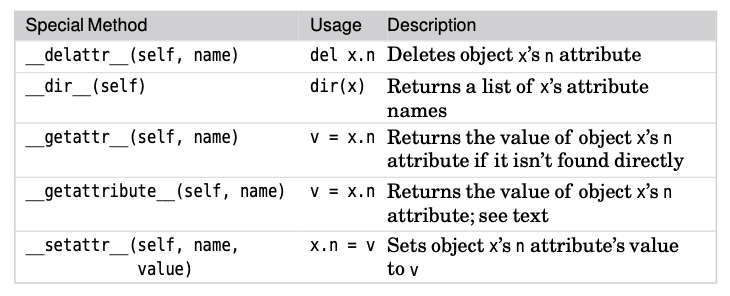
\includegraphics[width=\textwidth]{pics/attribute-special-methods}
  \caption{Attribute access speical methods}
  \label{fig:attribute-special-methods}
\end{figure}





If there are a lot of read-only properites, here is a different solution:
\begin{lstlisting}
USE_GETATTR = True


class Image:
    def __init__(self, width, height, filename="", background="#FFFFFF"):
        self.filename = filename
        self.__background = background
        self.__data = {}
        self.__width = width
        self.__height = height
        self.__colors = {self.__background}

    if USE_GETATTR:
        def __getattr__(self, name):
            if name == 'color':
                return set(self.__colors)
            classname = self.__class__.__name__
            if name in frozenset({'background', 'width', 'height'}):
                # image = Image(10, 10)
                # image.__dict__
                # {'filename': '',
                #  '_Image__background': '#FFFFFF',
                #  '_Image__data': {},
                #  '_Image__width': 10,
                #  '_Image__height': 10,
                #  '_Image__colors': {'#FFFFFF'}}
                return self.__dict__[f'_{classname}__{name}']
            raise AttributeError(f"'{classname}' object has no attribute {name}")
    else:
        @property
        def background(self):
            return self.__background

        @property
        def width(self):
            return self.__width

        @property
        def height(self):
            return self.__height

        @property
        def colors(self):
            return set(self.__colors)
\end{lstlisting}

If the variable \verb|USE_GETATTR| is true, \verb|__getattr__| is used to create read-only properites, otherwise the property decorator is used to create the read-only properties.

If we attemt to access an object's attribute and the attribute is not found, Python will call the \verb|__getattr__| method with the name of the attribute as a parameter.


There is a subtle difference in the that:
\begin{itemize}
\item using \verb|__getattr__()| provides access to the attribute in the instance's class (which may be subclass)
\item accessing the attribute directly uses the class the attribute is defined in 
\end{itemize}



Where as the \verb|__getattr__()| method is called last when looking for (nonspeical) attribute, the \verb|__getattribute__()| method is called first for every attribute access.
Although it can be useful or even essential in some cases to call \verb|__getattribute__()|, reimplementing the \verb|__getattribute__()| method can be tricky.


\subsection{Functors}

In Python, a \keyword{function object} is an object reference to any callable, such as a function, a lambda function, or a method.
The definition also includes classes, since an object reference to a class is a callable that, when called, returns an object of the given class.
In computer science a \keyword{functor} is an object that can be called as though it ware a function, so in Python terms a functor is just another kind of function object.
Any \keyword{class} that has a \verb|__call__()| special method is a functor.



The key benefit that functors offer is that they can maintain some state information.
\begin{lstlisting}
class Strip:
    def __init__(self, characters):
        self.characters = characters

    def __call__(self, string):
        return string.strip(self.characters)
  
strip_punctuation = Strip(',;:.!?')
print(strip_punctuation('Mike Chyson!'))  # Mike Chyson
\end{lstlisting}

We could achieve the same thing using a plain function or lambda, but if we need to store a bit more state or perform more complex processing, a functor is often the right solution.



A functor’s ability to capture state by using a class is very versatile and powerful,but sometimes it is more than we really need.
Another way to capture state is to use a \keyword{closure}.
\keyword{A closure is a function or method that captures some external state.}

\begin{lstlisting}
def make_strip_function(characters):
    def strip_function(string):
        return string.strip(characters)

    return strip_function  

strip_punctuation = make_strip_function(',;:.!?')
print(strip_punctuation('Mike Chyson!'))  # Mike Chyson

\end{lstlisting}

\begin{tcolorbox}
  If the state are complex, you can you a functor, otherwise you can use a plain function or lambda or closure.
\end{tcolorbox}

\subsection{Context manager}

\keyword{Context managers} allow us to simplify code by ensuring that certain operations are performed before and after a particular block of code is executed.
The behavior is achieved because context managers define two special methods, \verb|__enter__()| and \verb|__exit__()|, that Python treats specially in the scope of a \verb|with| statement.
When a context manager is created in a \verb|with| statement its \verb|__enter__()| method is automatically called, and
when the context manager goes out of scope after its with statement its \verb|__exit__()| method is automatically called.


The syntax for using context managers is:
\begin{tcolorbox}
\begin{verbatim}
with expression as variable
    suite
\end{verbatim}
\end{tcolorbox}

The \verb|expression| must be or must produce a context manager object;
if the optional \verb|as variable| part is specified, the variable is set to refer to the object returned by the context manager’s \verb|__enter__()| method (and this is often the context manager itself).
Because a context manager is guaranteed to execute its ``exit'' code (even in the face of exceptions), context managers can be used to eliminate the need for \verb|finally| blocks in many situations.
\keyword{The file objects returned by the built-in open() function are context managers.}


A file object is a context manager whose exit code always closes the file if it was opened.
The exit code is executed whether or not an exception occurs, but in the latter case, the exception is propagated.
This ensures that the file gets closed and we still get the chance to handle any errors.
For example:
\begin{lstlisting}
# without context manager
fh = None
try:
    fh = open(filename)
    for line in fh:
        process(line)
except EnvironmentError as err:
    print(err)
finally:
    if fh is not None:
        fh.close()

# with context manager
try:
    with open(filename) as fh:
        for line in fh:
            process(line)
except EnvironmentError as err:
    print(err)  
\end{lstlisting}

\begin{lstlisting}
try:
    with open(source) as fin, open(target, 'w') as fout:
        for line in fin:
            fout.write(process(line))
except EnvironmentError as err:
    print(err)  
\end{lstlisting}



If we want to create a custom context manager we must create a class that provides two methods: \verb|__enter__()| and \verb|__exit__()|.
Whenever a \verb|with| statement is used on an instance of such a class, the \verb|__enter__()| method is called and the return value is used for the \verb|as variable| (or thrown away if there isn’t one).
When control leaves the scope of the \verb|with| statement the \verb|__exit__()| method is called (with details of an exception if one has occurred passed as arguments).



Suppose we want to perform several operations on a list in an atomic manner.
For example, if we have a list of integers and want to append an integer, delete an integer, and change a couple of integers, all as a single operation, we could write code like this:
\begin{lstlisting}
try:
    with AtomicList(items) as atomic:
        atomic.append(1111)
        del atomic[3]
        atomic[8] = 2222
        atomic[index] = 3333
except (AttributeError, IndexError, ValueError) as err:
    print('no changes applied:', err)  
\end{lstlisting}


Here is the code for the AtomicList context manager:
\begin{lstlisting}
class AtomicList:
    def __init__(self, alist, shallow_copy=True):
        self.original = alist
        self.shallow_copy = shallow_copy

    def __enter__(self):
        self.modified = (self.original[:] if self.shallow_copy else copy.deepcopy(self.original))
        return self.modified

    def __exit__(self, exc_type, exc_val, exc_tb):
        if exc_type is None:  # exception type
            self.original[:] = self.modified  
\end{lstlisting}


If no exception occurred the \verb|exc_type| (``exception type'') will be \verb|None| and we know that we can safely replace the original list’s items with the items from the modified list.
(We cannot do \verb|self.original = self.modified| because that would just replace one object reference with another and would not affect the original list at all.
There is no \verb|return| in \verb|__exit__()|)
But if an exception occurred, we do nothing to the original list and the modified list is discarded.



The return value of \verb|__exit__()| is used to indicate whether any exception that occurred should be propagated.
A \verb|True| value means that we have handled any exception and so no propagation should occur.
Normally we always return \verb|False| or something that evaluates to \verb|False| in a Boolean context to allow any exception that occurred to propagate.
By not giving an explicit \verb|return| value, our \verb|__exit__()| returns \verb|None| which evaluates to \verb|False| and correctly causes any exception to propagate.



\subsection{Descriptors}

Descriptors are \keyword{classes} which provide access control for the attributes of other \keyword{classes}.
Any class that implements one or more of the descriptor special methods, \verb|__get__()|, \verb|__set__()|, and \verb|__delete__()|, is called (and can be used as) a descriptor.


The built-in \verb|property()| and \verb|classmethod()| functions are implemented using descriptors.
The key to understanding descriptors is that although we create an instance of a descriptor in a class as a class attribute, Python accesses the descriptor through the class's instances.



Let’s imagine that we have a class whose instances hold some strings.
We want to access the strings in the normal way, for example, as a property, but we also want to get an XML-escaped version of the strings whenever we want.
One simple solution would be that whenever a string is set we immediately create an XML-escaped copy.
But if we had thousands of strings and only ever read the XML version of a few of them, we would be wasting a lot of processing and memory for nothing.
So we will create a descriptor that will provide XML-escaped strings on demand \keyword{without storing them}.
Here's the client(owner) class, that is, the class uses the discriptor:


\begin{lstlisting}
class Product:
    __slots__ = ('__name', '__description', '__price')

    name_as_xml = XmlShadow('name')
    description_as_xml = XmlShadow('description')

    def __init__(self, name, description, price):
        self.__name = name
        self.__description = description
        self.__price = price

    @property
    def name(self):
        return self.__name

    @property
    def description(self):
        return self.__description

    @description.setter
    def description(self, description):
        self.__description = description

    @property
    def price(self):
        return self.__price

    @price.setter
    def price(self, price):
        self.__price = price

product = Product("Chisel <3cm>", "Chisel & cap", 45.25)
print(product.name, product.name_as_xml, product.description_as_xml, sep='\n')
# Chisel <3cm>
# Chisel &lt;3cm&gt;
# Chisel &amp; cap

\end{lstlisting}

The \verb|name_as_xml| and \verb|description_as_xml| class attributes are set to be instances of the \verb|XmlShadow| descriptor.
Although no \verb|Product| object has a \verb|name_as_xml| attribute or a \verb|description_as_xml| attribute, thanks to the descriptor we can write code like the previous.
This work because when we try to access, for example \verb|name_as_xml| attribute, Python finds that the \verb|Product| class has a descriptor with that name, and so uses the descriptor to get the attribute's value.

\begin{lstlisting}
from xml.sax.saxutils import escape

class XmlShadow:
    def __init__(self, attribute_name):
        self.attribute_name = attribute_name

    def __get__(self, instance, owner=None):
        return escape(getattr(instance, self.attribute_name))
\end{lstlisting}

When the \verb|name_as_xml| or \verb|description_as_xml| attribute is looked up, Python calls the descriptor's \verb|__get__()| method.
The \verb|self| argument is the instance of the descriptor, the \verb|instance| argument is the \verb|Product| instance, and the \verb|owner| argument is the owning class (\verb|Product| in this case).
We use the \verb|getattr()| function to retrieve the relevant attribute from the product (in this case the relevant property), and return an XML-escaped version of it.




If the use case was that only a small proportion of the products were accessed for their XML strings, but the strings were often long and the same ones were frequently accessed, we could use a cache.
\begin{lstlisting}
class CachedXmlShadow:
    def __init__(self, attribute_name):
        self.attribute_name = attribute_name
        self.cache = {}

    def __get__(self, instance, owner=None):
        xml_text = self.cache.get(id(instance))
        if xml_text is not None:
            return xml_text
        return self.cache.setdefault(id(instance), escape(getattr(instance, self.attribute_name)))
\end{lstlisting}

We store the unique identity of the instance as key rather than the instance itself because dictionary keys must be hashable, but we don't want to impose that as a requirement on classes that use the \verb|CachedXmlShadow| descriptor.
The key is necessary because descriptors are created per class rather than per instance.



Here's an example that use a descriptor to store all of an object's attrbute data, with the object not needing to store anything itself.

\begin{lstlisting}
class Point:
    # By setting __slots__ to an empty tuple we ensure that the class cannot store
    # any data attributes at all.
    __slots__ = ()
    x = ExternalStorage('x')
    y = ExternalStorage('y')

    def __init__(self, x=0, y=0):
        self.x = x
        self.y = y  
\end{lstlisting}

By setting \verb|__slots__| to an empty tuple we ensure that the class cannot store any data attributes at all.
When \verb|self.x| is assigned to, Python finds that there is a descriptor with the name ``x'', and so uses the descriptor's \verb|__set__()| method.


\begin{lstlisting}
class ExternalStorage:
    __slots__ = ('attribute_name',)
    __storage = {}  # class attribute

    def __init__(self, attribute_name):
        self.attribute_name = attribute_name

    def __set__(self, instance, value):
        self.__storage[id(instance), self.attribute_name] = value

    def __get__(self, instance, owner):
        if instance is None:
            d = {}
            for k in self.__storage.keys():
                if self.attribute_name in k:
                    d[k] = self.__storage[k]
            return d
        return self.__storage[id(instance), self.attribute_name]


p = Point(3, 4)
print(p.x, p.y)  # 3 4
p = Point(1, 2)
print(p.x, p.y)  # 1 2
print(Point.x, Point.y, Point, sep='\n')
# {(140338432304624, 'x'): 3, (140338432304640, 'x'): 1}
# {(140338432304624, 'y'): 4, (140338432304640, 'y'): 2}
# <class '__main__.Point'>

\end{lstlisting}

Although \verb|__storage| is a class attribute, we can access it as \verb|self.__storage|, because Python will look for it as an instance attribute, and not finding it will then look for it as a class attribute.

The implementation of the \verb|__get__()| special method is slightly more sophisticated than before because we provide a means by which all the attribute values in the ExternalStorage instance itself can be accessed.


We create the \verb|Property| descriptor that mimics the behavior of the built-in \verb|property()| function, at least for setters and getters.
Here's the class that makes use of it:
\begin{lstlisting}
class NameAndExtension:
    def __init__(self, name, extension):
        self.__name = name
        self.extension = extension

    @Property
    def name(self):
        return self.__name

    @Property
    def extension(self):
        return self.__extension

    @extension.setter
    def extension(self, extension):
        self.__extension = extension  
\end{lstlisting}


Here's the \verb|Property| decorator:
\begin{lstlisting}
class Property:
    def __init__(self, getter, setter=None):
        self.__getter = getter
        self.__setter = setter
        self.__name__ = getter.__name__

    def __get__(self, instance, owner=None):
        if instance is None:
            return self
        return self.__getter(instance)

    def __set__(self, instance, value):
        if self.__setter is None:
            raise AttributeError(f"'{self.__name__}' is read-only")
        return self.__setter(instance, value)

    def setter(self, setter):
        self.__setter = setter
        return self.__setter
\end{lstlisting}

The class's initializer takes one or two \keyword{functions} as arguments.
If it is used as a decorator, it will get just the decorated function and this becomes the getter, while the setter is set to \verb|None|.
We use the getter's name as the property's name.
So for each property, we have a getter, possiblely a setter, and a name.

When a property is accessed we return the result of calling the getter function where we have passed the instance as its first parameter.
At first sight, \verb|self.__getter()| looks like a method call, but is is not.
In face, \verb|self.__getter| is an attribute, one that happens to hold an object reference to a method that was passed.
So what happens is that first we retrieve the attribute (\verb|self__getter|), and then we call is as a function \verb|()|.
And because it is called as a function rather than a method we must pass in the relevant \verb|self| object explicitly ourselves.
And in the case of a descriptor the \verb|self| object is called \verb|instance|.

The \verb|setter()| method is called when the interpreter reaches, for example, \verb|@extension.setter|, with the function it decorates as its \verb|setter| argument.
It stores the setter method it has been given (which can now be used in the \verb|__set__()| method), and returns the setter, since decorator should return the function or method they decorate.


\subsection{Class decorators}

Class decorators takes a class object, and should return a class -- normally a modified version of the class they decorate.


\subsubsection{Example:  delegate}

Here's an example without class decorator:
\begin{lstlisting}
_identity = lambda x: x


class SortedList:
    def __init__(self, sequence=None, key=None):
        self.__key = key or _identity
        assert hasattr(self.__key, "__call__")
        if sequence is None:
            self.__list = []
        elif (isinstance(sequence, SortedList) and
              sequence.key == self.__key):
            self.__list = sequence.__list[:]
        else:
            self.__list = sorted(list(sequence), key=self.__key)

    def pop(self, index=-1):
        return self.__list.pop(index)

    def __delitem__(self, index):
        del self.__list[index]

    def __getitem__(self, index):
        return self.__list[index]

    def __setitem__(self, index, value):
        raise TypeError("use add() to insert a value and rely on "
                        "the list to put it in the right place")

    def __iter__(self):
        return iter(self.__list)

    def __reversed__(self):
        return reversed(self.__list)

    def __len__(self):
        return len(self.__list)

    def __str__(self):
        return str(self.__list)
\end{lstlisting}


Here's the decorated version:
\begin{lstlisting}
@delegate("__list", ("pop", "__delitem__", "__getitem__",
                     "__iter__", "__reversed__", "__len__", "__str__"))
class SortedList:

    def __init__(self, sequence=None, key=None):
        self.__key = key or _identity
        assert hasattr(self.__key, "__call__")
        if sequence is None:
            self.__list = []
        elif (isinstance(sequence, SortedList) and
              sequence.key == self.__key):
            self.__list = sequence.__list[:]
        else:
            self.__list = sorted(list(sequence), key=self.__key)
\end{lstlisting}

Here's class decorater:
\begin{lstlisting}
def delegate(attribute_name, method_names):
    def decorator(cls):
        nonlocal attribute_name
        if attribute_name.startswith('__'):
            attribute_name = '_' + cls.__name__ + attribute_name
        for name in method_names:
            setattr(cls, name, eval("lambda self, *a, **kw: "
                                    f"self.{attribute_name}.{name}(*a, **kw)"))
        return cls

    return decorator  
\end{lstlisting}

We could not use a plain decorator because we want to pass arguments to the decorator, so we have instead created a function that takes our arguments and then returns a class decorator.
The decorator itself takes a single argument, a class (just as a function decorator takes a single function or method as its argument).


We must use \verb|nonlocal| so that the nested function uses the \verb|attribute_name| from the outer scope rather than attempting to use one from its own scope.
And we must be able to correct the attribute name if necessary to take account of the name mangling of private attributes.
The decorator’s behavior is quite simple:
It iterates over all the method names that the \verb|delegate()| function has been given, and for each one creates a new method which it sets as an attribute on the class with the given method name.


We have used \verb|eval()| to create each of the delegated methods since it can be used to execute a single statement, and a \verb|lambda| statement produces a method or function.
For example, the code executed to produce the \verb|pop()| method is:
\begin{lstlisting}
lambda self, *a, **kw: self._SortedList__list.pop(*a, **kw)  
\end{lstlisting}


\subsubsection{Example: complete comparisons}


In the following example, only \verb|__lt__()| special method is supplied, and the other comparison method is created by the class decorator.
\begin{lstlisting}
@complete_comparisons
class FuzzyBool:
    def __init__(self, value=0.0):
        self.__value = value if 0.0 <= value <= 1.0 else 0.0

    def __lt__(self, other):
        return self.__value < other.__value
\end{lstlisting}


Here's the decorator:
\begin{lstlisting}
def complete_comparisons(cls):
    assert cls.__lt__ is not object.__lt__, (
        f'{cls.__name__} must define < and ideally =='
    )
    if cls.__eq__ is object.__eq__:
        cls.__eq__ = lambda self, other: (
            not (cls.__lt__(self, other) or cls.__lt__(other, self))
        )
    cls.__ne__ = lambda self, other: not cls.__eq__(self, other)
    cls.__gt__ = lambda self, other: cls.__lt__(other, self)
    cls.__le__ = lambda self, other: not cls.__lt__(other, self)
    cls.__ge__ = lambda self, other: not cls.__lt__(self, other)
\end{lstlisting}


Given a class that defines only < (or < and ==), the decorator produces the missing comparison operators by using the following logical equivalences:
\begin{figure}[H]
  \centering
  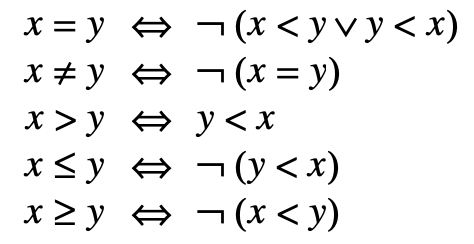
\includegraphics[width=\textwidth]{pics/logical-equivalences}
  \caption{Logical equivalences}
\end{figure}


In fact, Python automatically produces > if < is supplied, != if == is supplied, and >= if <= is supplied, so it is sufficient to just implement the three operators <, <=, and == and to leave Python to infer the others.
However, using the class decorator reduces the minimum that we must implement to just <.
This is convenient, and also ensures that all the comparison operators use the same consistent logic.


One problem that the decorator faces is that class \verb|object| from which every other class is ultimately derived defines all six comparison operators, all of which raise a \verb|TypeError| exception if used.
So we need to know whether < and == have been reimplemented (and are therefore usable).
This can easily be done by comparing the relevant special methods in the class being decorated with those in \verb|object|.



\begin{tcolorbox}
  Using class decorators is probably the simplest and most direct way of changing classes. Another approach is to use metaclasses.
\end{tcolorbox}



\subsection{Abstract base classes}

An abstract base class (ABC) is a class that \keyword{cannot be used to create objects}.
Instead, the purpose of such classes is \keyword{to define interface}, that is, to in effect list the methods and properites that classes that inherit the abstract base class must provide.
This is useful because we can use an abstract base class as a kind of \keyword{promise} -- a promise that any derived class will provide the methods and properites that the abstract base class specifies.


\begin{tcolorbox}
  Abstract base classes are classes that have at least one abstract method or property.
\end{tcolorbox}

\begin{tcolorbox}
  All ABCs must have a metaclass of \verb|abc.ABCMeta| (from the \verb|abc| module), or from one of its subclasses.
\end{tcolorbox}





\subsubsection{Example:  Appliance}

\begin{lstlisting}
import abc


class Appliance(metaclass=abc.ABCMeta):
    @abc.abstractmethod
    def __init__(self, model, price):
        self.__model = model
        self.price = price

    def get_price(self):
        return self.__price

    def set_price(self, price):
        self.__price = price

    price = abc.abstractproperty(get_price, set_price)

    @property
    def model(self):
        return self.__model  
\end{lstlisting}


We have set the class’s metaclass to be \verb|abc.ABCMeta| since this is a requirement for ABCs.
We have made \verb|__init__()| an abstract method to ensure that it is reimplemented, and we have also provided an implementation which we expect (but can’t force) inheritors to call. 
To make an abstract readable/writable property we cannot use decorator syntax; also we have not used private names for the getter and setter since doing so would be inconvenient for subclasses.


The \verb|price| property is abstract (so we cannot use the \verb|@property| decorator), and is readable/wriable data as a property.
We initialize the \keyword{property} in the \verb|__init__()| method rather than setting the private data directly --
this ensures that the setter is called (and may potentially do validation or other work, although it doesn’t in this particular example).



The \verb|model| property is not abstract, so subclasses don’t need to reimplement it, and we can make it a property using the \verb|@property| decorator.



Here is an example subclass:
\begin{lstlisting}
class Cooker(Appliance):
    def __init__(self, model, price, fuel):
        super().__init__(model, price)
        self.fuel = fuel

    price = property(lambda self: super().price,
                     lambda self, price: super().set_price(price))  
\end{lstlisting}


\subsubsection{Example: TextFilter}

\begin{lstlisting}
import abc


class TextFilter(metaclass=abc.ABCMeta):
    @abc.abstractmethod
    def is_tranformer(self):
        raise NotImplementedError()

    @abc.abstractmethod
    def __call__(self):
        raise NotImplementedError()  
\end{lstlisting}

The \verb|TextFilter| ABC provides no functionality at all; it exists purely to define an interface.
Since the abstract property and method have no implementations we don’t want subclasses to call them, so instead of using an innocuous pass statement we raise an exception if they are used



Here are some subclasses:
\begin{lstlisting}
class CharCounter(TextFilter):
    @property
    def is_tranformer(self):
        return False

    def __call__(self, text, chars):
        count = 0
        for c in text:
            if c in chars:
                count += 1
        return count


class RunLengthEncoder(TextFilter):
    @property
    def is_tranformer(self):
        return True

    def __call__(self, utf8_string):
        byte = None
        count = 0
        binary = bytearray()
        for b in utf8_string.encode("utf8"):
            if byte is None:
                if b == 0:
                    binary.extend((0, 1, 0))
                else:
                    byte = b
                    count = 1
            else:
                if byte == b:
                    count += 1
                    if count == 255:
                        binary.extend((0, count, b))
                        byte = None
                        count = 0
                else:
                    if count == 1:
                        binary.append(byte)
                    elif count == 2:
                        binary.extend((byte, byte))
                    elif count > 2:
                        binary.extend((0, count, byte))
                    if b == 0:
                        binary.extend((0, 1, 0))
                        byte = None
                        count = 0
                    else:
                        byte = b
                        count = 1
        if count == 1:
            binary.append(byte)
        elif count == 2:
            binary.extend((byte, byte))
        elif count > 2:
            binary.extend((0, count, byte))
        return bytes(binary)


class RunLengthDecoder(TextFilter):
    @property
    def is_tranformer(self):
        return True

    def __call__(self, rle_bytes):
        binary = bytearray()
        length = None
        for b in rle_bytes:
            if length == 0:
                length = b
            elif length is not None:
                binary.extend([b for x in range(length)])
                length = None
            elif b == 0:
                length = 0
            else:
                binary.append(b)
                length = None
        if length:
            binary.extend([b for x in range(length)])
        return binary.decode("utf8")


if __name__ == '__main__':
    vowel_counter = CharCounter()
    count = vowel_counter('dog fish and cat fish', 'aeiou')
    print(count)  # 5

    print('=' * 100)
    text = 'Mack Chyson ======================='
    encoder = RunLengthEncoder()
    encoded_text = encoder(text)
    print(encoded_text)  # b'Mack Chyson \x00\x17='
    decoder = RunLengthDecoder()
    original_text = decoder(encoded_text)
    print(original_text)
    # Mack Chyson =======================
\end{lstlisting}


\subsubsection{Example: Abstract}

\begin{lstlisting}
class Undo(metaclass=abc.ABCMeta):
    @abc.abstractmethod
    def __init__(self):
        self.__undos = []

    @abc.abstractmethod
    def can_undo(self):
        return bool(self.__undos)

    @abc.abstractmethod
    def undo(self):
        assert self.__undos, 'nothing left to undo'
        self.__undos.pop()(self)

    def add_undo(self, undo):
        self.__undos.append(undo)

    def clear(self):
        self.__undos = []  
\end{lstlisting}

The \verb|self.__undos| list is exprected to hold object references to methods.
Each method must cause the corresponding action to be undone if it is called.
So to perform an undo we pop the last undo method off the \verb|self.__undos| list, and then call the method as a function, passing \verb|self| as an argument.
(We must pass \verb|self| because the method is being called as a function not at a method.)


Here's \verb|Stack| class:
\begin{lstlisting}
class Stack(Undo):
    def __init__(self):
        super().__init__()
        self.__stack = []

    @property
    def can_undo(self):
        return super().can_undo

    def undo(self):
        super().undo()

    def push(self, item):
        self.__stack.append(item)
        self.add_undo(lambda self: self.__stack.pop())

    def pop(self):
        item = self.__stack.pop()
        self.add_undo(lambda self: self.__stack.append(item))
        return item

    def top(self):
        assert self.__stack, 'Stack is empty'
        return self.__stack[-1]

    def __str__(self):
        return str(self.__stack)
\end{lstlisting}


\subsection{Multiple inheritance}

Multiple inheritance is where one class inherits from two or more other classes.
One problem is that multiple inheritance can lead to the same class being inherited more than once and this means that the version of a method that is called depends on the method resolution order,
which potentially makes classes that use multiple inheritance somewhat fragile.



Multiple inheritance can generally ba avoided by:
\begin{itemize}
\item Using single inheritance and setting a metaclass if we want to support an additional API
\item Using mutiple inheritance with one concrete class and one or more abstract base classes for addtional APIs
\item Using single inheritance and aggregate instances of other classes
\end{itemize}





Nonetheless, in some cases, multiple inheritance can provide a very convenient solution.
For example, suppose we want to create a new version of the \verb|Stack| class from the previous subsection, but want the class to support loading and saving using a pickle.
We might well want to add the loading and saving functionality to several classes, so we will implement it in a class of its own:
\begin{lstlisting}
class LoadSave:
    def __init__(self, filename, *attribute_names):
        self.filename = filename
        self.__attribute_names = []
        for name in attribute_names:
            if name.startswith('__'):
                name = '_' + self.__class__.__name__ + name
            self.__attribute_names.append(name)

    def save(self):
        with open(self.filename, 'wb') as fh:
            data = []
            for name in self.__attribute_names:
                data.append(getattr(self, name))
            pickle.dump(data, fh, pickle.HIGHEST_PROTOCOL)

    def load(self):
        with open(self.filename, 'rb') as fh:
            data = pickle.load(fh)
            for name, value in zip(self.__attribute_names, data):
                setattr(self, name, value)
  
\end{lstlisting}


\begin{lstlisting}
class FileStack(Undo, LoadSave):
    def __init__(self, filename):
        Undo.__init__(self)
        LoadSave.__init__(self, filename, '__stack')
        self.__stack = []

    def load(self):
        super().load()
        Undo.clear(self)
\end{lstlisting}

Instead of using \verb|super()| in the \verb|__init__()| method we must specify the base classes that we initialize since \verb|super()| cannot guess out intensions.


\begin{tcolorbox}
  Multiple inheritance can be convenient and works well when the inheritance classes have no overlapping APIs.
\end{tcolorbox}



\subsection{Metaclasses}

A metaclass is to a class what a class is to an instance; that is, a metaclass is used to create classes, just as classes are used to create instances.
We can ask whether a class object inherits another class using \verb|issubclass()|.


\subsubsection{Register}


The simplest use of metaclasses is to make custom classes fit into Python's standard ABC hierarchy.

\begin{lstlisting}
import collections


class SortedList:
    pass


collections.abc.Sequence.register(SortedList)
\end{lstlisting}


Registering a class like this makes it a \keyword{virtual subclass}.
A virtual subclass reports that it is a subclass of the class or classes it it registed with, but does not inherit any data or methods from any of the classes it is registered with.
Registering a class like this provides a promise that the class provides the API of the classes it is registered with, but does not provide any guarantee that it will honor its promise.


\subsubsection{Guarantee}


One use of metaclasses is to provide both a promise and a guarantee about a class's API.
Another use is to modify a class in some way (like a class decorator does).
And metaclasses can be used for both purposes at the same time.



Suppose we want to create a group of classes that all provide \verb|load()| and \verb|save()| methods.
We can do this by creating a class that when used as a metaclass, checks that these methods are present:

\begin{lstlisting}
# API guarantee
class LoadableSavable(type):
    def __init__(cls, classname, bases, dictionary):
        super().__init__(classname, bases, dictionary)

        assert (
            hasattr(cls, 'load') and
            isinstance(getattr(cls, 'load')), collections.abc.Callable
        ), "class '" + classname + "' must provide a load() method"
        assert (
                hasattr(cls, 'save') and
                isinstance(getattr(cls, 'save'), collections.abc.Callable)
        ), "class '" + classname + "' must provide a save() method"
\end{lstlisting}



Classes that are to serve as metaclasses must inherit from the ultimate metaclass base class, \verb|type|, or one of its subclasses.


Once the class has been created, the metaclass is initialized by calling its \verb|__init__()| method.
The arguments given to \verb|__init__()| are \verb|cls|, the class that just been created;
\verb|classname|, the class's name;
\verb|bases|, a list of the class's base classes (excluding \verb|object|, and therefore possibly empty);
and \verb|dictionary| that holds the attributes that became class attributes when the \verb|cls| class was created,
unless we intervened in a reimplementation of the metaclass's \verb|__new__()| method.



\begin{lstlisting}
# class Bad(metaclass=LoadableSavable):
#     def some_method(self): pass
# AssertionError: class 'Bad' must provide a load() method

class Good(metaclass=LoadableSavable):
    def load(self): pass
    def save(self): pass


g = Good()
\end{lstlisting}



\subsubsection{Modify}

We can use metaclasses to change the classes use them.
If the change involves the name, base classes, or dictionary of the class being created, the we need to reimplement the metaclass's \verb|__new__()| method;
buf for other changes, such as adding methods or data attributes, reimplementing \verb|__init__()| is sufficient, although this can also be done in \verb|__new__()|.





This exmaple is just used to show the modification function.
Normall the following code is not good.
Suppose we did not use property decorators before, but use a simple naming convetion ti identify properties.
Here, the class has methods of the form \verb|get_name()| and \verb|set_name()|, we would expect the class to have a private \verb|__name| property accessed using \verb|instance.name| for getting and setting.
Here is the class:

\begin{lstlisting}
class Product(metaclass=AutoSlotProperties):
    def __init__(self, barcode, description):
        self.__barcode = barcode
        self.description = description

    def get_barcode(self):
        return self.__barcode

    def get_description(self):
        return self.__description

    def set_description(self, description):
        if description is None or len(description) < 3:
            self.__description = '<Invalid Description>'
        else:
            self.__description = description
\end{lstlisting}

This can be done using a metaclass.

\begin{lstlisting}
# modifying properties
class AutoSlotProperties(type):
    def __new__(mcl, classname, bases, dictionary):
        slots = list(dictionary.get('__slot__', []))  # get slots
        for getter_name in [key for key in dictionary if key.startswith('get_')]:
            if isinstance(dictionary[getter_name], collections.abc.Callable):
                name = getter_name[4:]
                slots.append('__' + name)  # alter slots
                getter = dictionary.pop(getter_name)
                setter_name = 'set_' + name
                setter = dictionary.get(setter_name, None)
                if setter is not None and isinstance(setter, collections.abc.Callable):
                    del dictionary[setter_name]
                dictionary[name] = property(getter, setter)  # convert to property
        dictionary['__slots__'] = tuple(slots)
        return super().__new__(mcl, classname, bases, dictionary)  



product = Product('111', '8mm Stapler')
print(product.barcode, product.description)  # 111 8mm Stapler
product.description = '8mm Stapler (long)'
print(product.barcode, product.description)  # 111 8mm Stapler (long)

print(product.__slots__)  # ('__barcode', '__description')

for i in dir(product):
    print(i)
# _Product__barcode
# _Product__description
# __class__
# __delattr__
# __dir__
# __doc__
# __eq__
# __format__
# __ge__
# __getattribute__
# __gt__
# __hash__
# __init__
# __init_subclass__
# __le__
# __lt__
# __module__
# __ne__
# __new__
# __reduce__
# __reduce_ex__
# __repr__
# __setattr__
# __sizeof__
# __slots__
# __str__
# __subclasshook__
# barcode
# description  
\end{lstlisting}



\section{Functional-style programming}


Functional-style programming is an approach to programming where computations are built up from combining functions:
\begin{itemize}
\item tha don't modify their arguments and 
\item that don't refer to or change the program's state, and 
\item that provide their results as return values.
\end{itemize}



Three concepts that are strongly associated with functional programming are
\begin{enumerate}
\item mapping
\item filtering
\item reducing
\end{enumerate}


Mapping involves taking a function and an iterable and producing a new iterable (or a list) where each item is the result of calling the function on the corresponding item in the original iterable.
This is supported by the built-in \verb|map()| function, for example:
\begin{lstlisting}
list(map(lambda x: x ** 2, [1, 2, 3, 4]))
Out[3]: [1, 4, 9, 16]  
\end{lstlisting}



Filtering involves taking a function and an iterable and producing a new iterable where each item is from the original iterable -- providing the function returns True when called on the item.
The built-in \verb|filter()| function supports this:
\begin{lstlisting}
list(filter(lambda x: x > 0, [1, -2, 3, -4]))
Out[5]: [1, 3]  
\end{lstlisting}


Reducing involves taking a function and an iterable and producing a single result value.
The way this works is that the function is called on the iterable’s first two values, then on the computed result and the third value, then on the computed result and the fourth value, and so on, until all the values have been used. 
The \verb|functools| module's \verb|functools.reduce()| function supports this.
\begin{lstlisting}
import functools
functools.reduce(lambda x, y: x * y, [1, 2, 3, 4])
Out[7]: 24
import operator
functools.reduce(operator.mul, [1, 2, 3, 4])
Out[9]: 24
\end{lstlisting}


The \verb|operator| module has functions for all of Python’s operators specifically to make functional-style programming easier. 





Python provides some built-in reducing functions:
\begin{description}
\item[all()] given an iterable, returns \verb|True| if all the iterable’s items return \verb|True| when \verb|bool()| is applied to them;
\item[any()] returns \verb|True| if any of the iterable’s items is \verb|True|;
\item[max()] returns the largest item in the iterable;
\item[min()] returns the smallest item in the iterable; 
\item[sum()] returns the sum of the iterable’s items.
\end{description}




\subsection{Partial function application}

Partial function application is the creation of a function from an existing function and some arguments to produce a new function that does what the original function did, but with some arguments fixed so that callers don’t have to pass them.
Here’s a very simple example:
\begin{lstlisting}
enumerate1 = functools.partial(enumerate, start=1)
for lino, line in enumerate1(lines):
    process_line(lino, line)
\end{lstlisting}



Using partial function application can simplify our code, especially when we want to call the same functions with the same arguments again and again.
For example:

\begin{lstlisting}
reader = functools.partial(open, mode='rt', encoding='utf8')
writer = functools.partial(open, mode='wt', encoding='utf8')
\end{lstlisting}

\begin{lstlisting}
Conv2D_ = functools.partial(Conv2D, kernel_size=(3, 3), activation='relu', padding='same')

h = Conv2D_(256)(input_layer)
h = Conv2D_(64)(h)

# The same full code is:
# h = Conv2D(256, (3, 3), activation='relu', padding='same')(input_layer)
# h = Conv2D(64, (3, 3), activation='relu', padding='same')(h)  
\end{lstlisting}


\subsection{Coroutines}

Coroutines are functions whose processing can be suspended and resumed at specific points.


In Python, a coroutine is a function that takes its input from a \verb|yield| expression.
It may also send results to a receiver function (which itself must be a coroutine).
Whenever a coroutine reaches a \verb|yield| expression it suspends waiting for data; and once it receives data, it resumes execution from that point.


\subsubsection{Composing pipelines}

A pipeline is simply the composition of one or more functions where data items are sent to the first function, which then either discards the item (filters it out) or passes it on to the next function (either as is or transformed in some way).
The second function receives the item from the first function and repeats the process, discarding or passing on the item (possibly transformed in a different way) to the next function, and so on.
Items that reach the end are then output in some way.


\begin{tcolorbox}
One benefit of using pipelines is that we can read data items incrementally, often one at a time, and have to give the pipeline only enough data items to fill it (usually one or a few items per component).
This can lead to significant \keyword{memory savings} compared with, say, reading an entire data set into memory and then processing it all in one go.  
\end{tcolorbox}



Here is an example -- a file matcher that reads all the filenames given on the command line (including those in the directories given on the command line, recursively), and that output the absolute paths of those files that meet certain criteria.




\begin{lstlisting}
import os
import sys
import functools


def coroutine(function):
    @functools.wraps(function)
    def wrapper(*args, **kwargs):
        generator = function(*args, **kwargs)
        next(generator)
        return generator

    return wrapper


@coroutine
def reporter():
    while True:
        filename = (yield)
        print(filename)


@coroutine
def get_files(receiver):
    """
    A wrapper of os.walk()
    :param receiver:
    :return:
    """
    while True:
        path = (yield)
        if os.path.isfile(path):
            receiver.send(os.path.abspath(path))
        else:
            for root, dirs, files in os.walk(path):
                for filename in files:
                    receiver.send(os.path.abspath(os.path.join(root, filename)))


@coroutine
def suffix_matcher(receiver, suffixes):
    while True:
        filename = (yield)
        if filename.endswith(suffixes):
            receiver.send(filename)


@coroutine
def size_matcher(receiver, minimum=None, maximum=None):
    while True:
        filename = (yield)
        size = os.path.getsize(filename)
        if ((minimum is None or size >= minimum) and
                (maximum is None or size <= maximum)):
            receiver.send(filename)


if __name__ == '__main__':
    # notice the order in coroutine
    pipes = []
    pipes.append(reporter)
    pipes.append(size_matcher(pipes[-1], minimum=1024))
    pipes.append(suffix_matcher(pipes[-1], (".png", ".jpg", ".jpeg", ".py")))
    pipes.append(get_files(pipes[-1]))
    pipeline = pipes[-1]
    # Equal to
    # pipeline = get_files(suffix_matcher(size_matcher(reporter(), minimum=1024), (".png", ".jpg", ".jpeg", ".py")))

    try:
        for file in sys.argv[1:]:
            print(file)
            pipeline.send(file)
            # pipeline.py
            # /Users/mike/PycharmProjects/python3/c8_advanced_programming_techniques/functional_programming/pipeline.py
            # partial.py
            # /Users/mike/PycharmProjects/python3/c8_advanced_programming_techniques/functional_programming/partial.py
            # __init__.py
    finally:
        for pipe in pipes:
            pipe.close()
  
\end{lstlisting}

The \verb|@coroutine| decorator takes a coroutine function, and calls the built-in \verb|next()| function on it -- this causes the function to be executed up to the first \verb|yield| expression, ready to receive data.




